\subsection{Data Set}
\subsubsection{Stock Selection}

For our prediction model, we carefully selected approximately 15 stocks from both the KODEX 200 and S\&P 500 indices \cite{KRX}\cite{NASDAQ}.
o add a layer of analysis, we categorized these stocks into two distinct groups: stable and unstable. 
This categorization was based on their presence in commercial ETF fund holdings. 
The table\ref{tab:example} below details the specific stocks chosen for our study.

\begin{table}[h]
	\label{tab:example}
	\tiny
	\centering
	\begin{tabular}{cc}
	\toprule\toprule
	\textbf{Korea} & \textbf{Korea} \\ 
	\textbf{Stable} & \textbf{unstable}  \\ 
	\midrule
	Samsung Electronics Co Ltd					&	Posco Holdings Inc				\\
	Samsung SDI Co Ltd							&	Naver Corp						\\
	KT\&G Corp									&	Hyundai Motor Co				\\
	Yuhan Corp									&	LG Chem Ltd						\\
	SK Hynix Inc								&	Kia Corp						\\
	DB Insurance Co Ltd							&	Celltrion Inc					\\
	Korea Zinc Inc								&	KB Financial Group Inc			\\
	Fila Holdings Corp							&	Shinhan Financial Group Co Ltd	\\
	Meritz Financial Group Inc					&	LG Energy Solution Ltd			\\
	Cheil Worldwide Inc							&	Kakao Corp						\\
	LG Innotek Co Ltd							&	HYUNDAI MOBIS CO., LTD.			\\
	Shinsegae Inc								&	Samsung C\&T Corp				\\
	IBK											&	Samsung Biologics Co Ltd		\\
	NCSoft Corp									&	LG Electronics Inc				\\
	Lotte Chemical Corp							&	Hana Financial Group Inc		\\
	Leeno Industrial Inc						&									\\
	Nongshim Co Ltd								&									\\
	S1 Corp										&									\\
	Hyundai Marine \& Fire Insurance Co. Ltd.	&									\\
	\midrule
	\textbf{US Nasdaq} & \textbf{US Nasdaq} \\ 
	\textbf{Stable} & \textbf{unstable} \\ 
	\midrule
	Coca-Cola Co					&	Apple Inc											\\
	McDonald's Corp					&	Microsoft Corp										\\
	Waste Management, Inc.			&	Amazon.com Inc										\\
	Republic Services Inc			&	NVIDIA Corp											\\
	PepsiCo, Inc.					&	Meta Platforms Inc									\\
	Colgate-Palmolive Company		&	Broadcom Inc										\\
	Walmart Inc						&	Alphabet Inc Class A								\\
	Cboe Global Markets Inc			&	Alphabet Inc Class C								\\
	General Dynamics Corp			&	Tesla Inc											\\
	Kimberly-Clark Corp				&	Adobe Inc											\\
	Procter \& Gamble Co			&	Costco Wholesale Corporation						\\
	Cencora Inc						&	Cisco Systems Inc									\\
	IBM Common Stock				&	Netflix Inc											\\
									&	Advanced Micro Devices, Inc.						\\
	\bottomrule
	\end{tabular}
	\caption{Stocks selected for our study}
\end{table}

\subsubsection{Normalization}

To standardize the stock price data for analysis, we applied a normalization process. Let $P_{t}$ be the stock price of the $t$-th day, and $P_{i}^{\prime}$ denote the normalized stock price on the same day. The normalization formula is as follows:
Then, we have
\begin{equation}
	P_{t}^{\prime} = \frac{P_{t}}{P_{\max} - P_{\min}}
\end{equation}
where $P_{max}$ and $P_{min}$ are the maximum and minimum stock prices within the specified period, respectively. This normalization allows for a more consistent comparison across different stocks and time frames.

\subsubsection{Training Set}

Our training dataset comprises various stock price metrics—open price, close price, high price, and low price—from the period of 2021 to 2022. 
Due to challenges in sourcing older news articles necessary for VADER analysis, the timeframe for our training data is thus constrained.

\subsubsection{Test Set}

For testing, we utilized stock price data (including open, close, high, and low prices) from the period of February 17, 2023, to December 1, 2023. 
Our testing approach involved using a set of 30 days' worth of stock prices and sentiment scores to predict the stock price for the subsequent day.

\subsection{UI/UX Design}
The user experience (UX) and user interface (UI) aspects of the system were prioritized to ensure a seamless and intuitive user interaction. 
The frontend was designed with a user-centric approach, focusing on usability and visual appeal.
% User research and feedback were considered to create an intuitive navigation flow, clear information hierarchy and visually pleasing design elements. 
The UI elements were designed to be responsive and accessible across different devices and screen sizes, enhancing the overall user experience.



\subsection{Frontend}
\begin{figure}
	\centering
	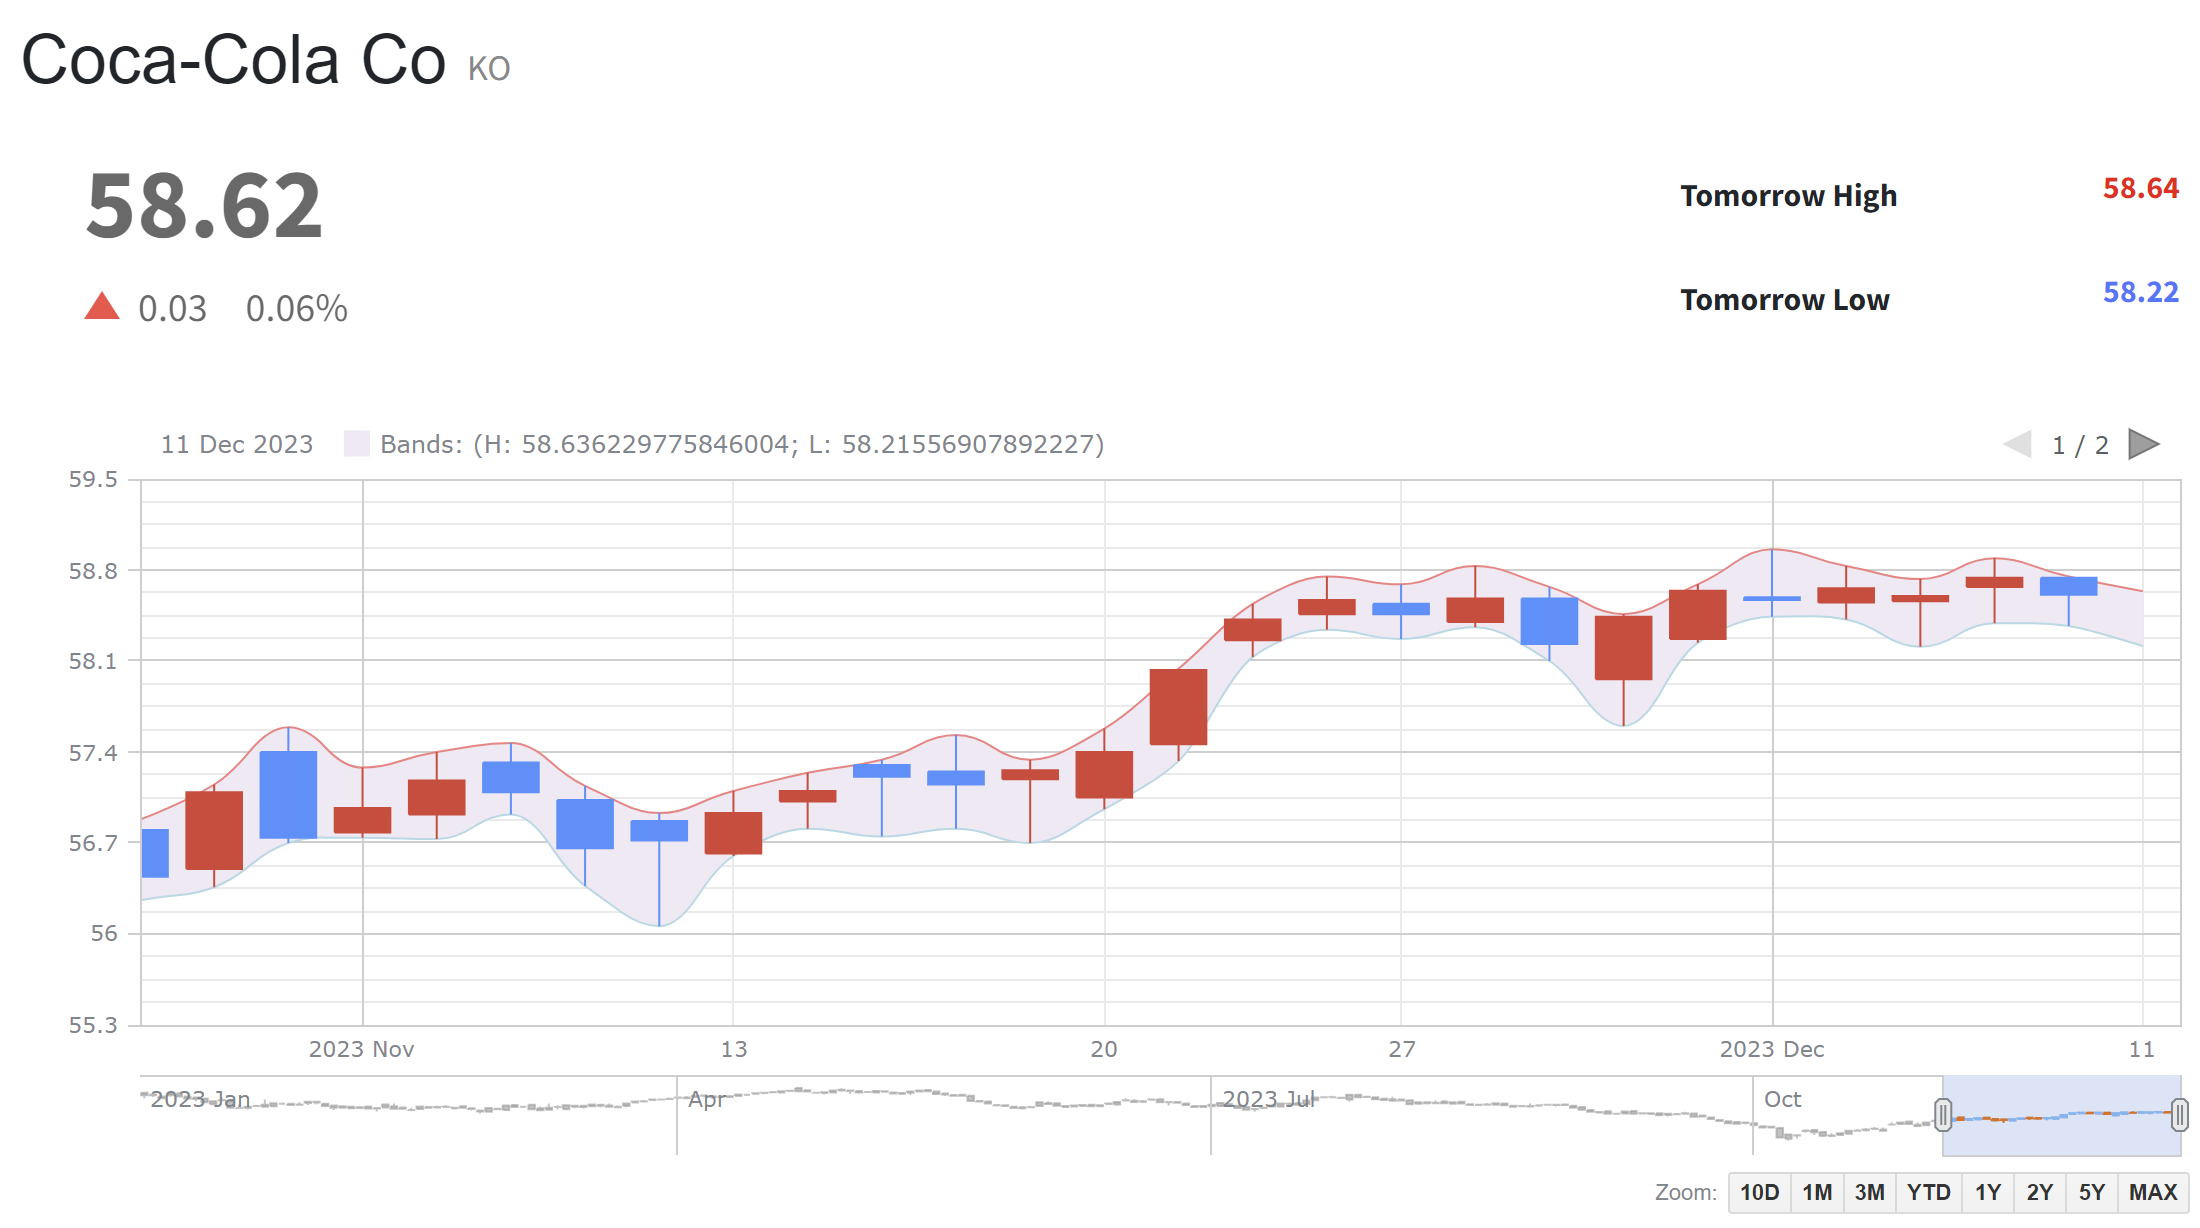
\includegraphics[width=0.8\textwidth]{Fig/Front.png}
	\caption{UI design of the main page}
	\label{fig:fig1}
\end{figure}

The frontend development involved translating the UI designs into HTML and CSS code.
JavaScript was used for client-side scripting and implementing interactive features as seen in the Figure \ref{fig:fig1}.
We employ anychart packages for visualizing stock price data.


\subsection{Backend}
Django, a Python web framework, was employed for server-side development.
It enables us to build a robust and scalable backend server, which is essential for our project.
We chose to use AWS EC2 instance, t2.micro, with 1GB RAM, 1 vCPU, as it offers a lightweight and suitable solution for our initial deployment.